\section{Motivation}
Sucht man im Internet Nachrichten über das Thema Erdbeben, wird schnell ersichtlich, dass beinahe jeden Tag ein ernstzunehmendes Erdbeben auftritt. Sucht man weiterhin nach einer zuverlässigen Vorhersage für Erdbeben, stellt man ebenso schnell fest, dass dies zurzeit noch nicht möglich ist.\\
Mittels der Umsetzung eines verteilten Erdbebenwarnsystems ist die Warnung zwar auch erst möglich, wenn das Erdbeben bereits spürbar ist, da sich Erdbeben jedoch vom Epizentrum aus ausbreiten, können umliegende Bereiche noch von einer Warnung profitieren. Zudem könnten, wie bereits im Abstract beschrieben, Sicherheitsmaßnahmen in Gang gesetzt werden.
Für das verteilte Erdbebensystem ist Android als Plattform ausgewählt worden. Dies begründet sich in der großen Verbreitung des Systems, welche momentan bei über 64\% weltweit liegt\footnote{http://techcrunch.com/2013/04/28/android-picks-up-the-pace-in-smartphone-sales-over-ios-globally-while-windows-phone-continues-with-modest-gains-says-kantar/}. 
\begin{figure}[H]
\centering
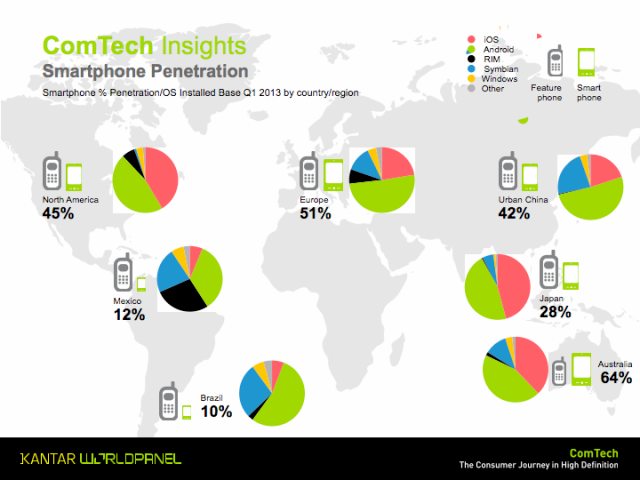
\includegraphics[width=\textwidth]{/AndroidVerbreitung.png}
\caption{Smartphone Betriebssystem-Verbreitung}
\label{fig:AndroidVerbreitung}
\end{figure}
